\chapter{Classical results in mathematical epidemiology}


Epidemics are typical examples of complex phenomena. A mathematical description of an epidemic needs to take into account its non deterministic nature, and, therefore, rely on probabilities. An epidemic process is, essentially, a stochastic process. 

In the dawn of mathematical epidemiology, researchers studied the dynamics in time of probabilities regarding the states of individuals. This is the case of  the study of life expectancy and smallpox by Daniel Bernoulli, and so is the famous contribution of Kermac y McEndrick with the SIR models. In both cases, the resulting dynamic equations correspond to the Master equation of the given stochastic processes.


\section{A supersonic intro to Master equation}

%\section{Stochastic processes and Master equation}

\subsection*{Introduction to Stochastic Processes and Markov Chains}

A \textbf{stochastic process} is a mathematical model that describes the evolution of a random system over time. It's a collection of random variables indexed by time, and can be used to model a wide range of phenomena, from the stock market to the weather.

A \textbf{Markov chain} is a specific type of stochastic process that has the \textbf{Markov property}: the future state of the system only depends on the current state, and not on any of the previous states. This makes Markov chains particularly useful for modeling systems where the future is dependent on the present, but not on the past.

Formally, a Markov chain is a sequence of random variables $X_0, X_1, X_2, \ldots$ that take values in a finite or countable set $S$, where the probability of moving from one state to another depends only on the current state. That is, for all $n \geq 0$ and all states $i, j \in S$,

\begin{equation*}
    \mathbb{P}(X_{t+1} = j \mid X_t = i, X_{t-1} = i_{t-1}, \ldots, X_0 = i_0) = \mathbb{P}(X_{t+1} = j \mid X_t = i).
\end{equation*}

Markov chains have many interesting properties and applications, including their use in modeling queueing systems, random walks, and machine learning algorithms.


\subsection*{Master equation}

The Master Equation is a fundamental tool in the study of stochastic processes, particularly in probability theory and statistical physics. It describes the time evolution of the probability distribution of a system in terms of transition rates between different states. In its simplest form, the Master Equation takes the form of a first-order differential equation:

\begin{equation}
    \frac{d}{dt} P_i(t) = \sum_j W_{ji} P_j(t) - \sum_j W_{ij} P_i(t),
\end{equation}
where $P_i(t)$ is the probability of the system being in state $i$ at time $t$, and $W_{ij}$ is the transition rate from state $j$ to state $i$. The first term on the right-hand side of the equation represents the rate of transitions from all other states $j$ to state $i$, weighted by the probability of being in state $j$. The second term represents the rate of transitions from state $i$ to all other states $j$, weighted by the probability of being in state $i$.

Master equation can be seen as a continuity equation, or a mass conservation equation. In fluid dynamics, for instance, the rate of change of mass in a control volume must be equal to the net rate of mass flow into or out of the control volume. Mathematically, the continuity equation can be written as:
$$\frac{\partial \rho}{\partial t} + \nabla \cdot (\rho \mathbf{v}) = \qquad \frac{d}{dt} \int_V   \rho \: \ud V +  \oint_S  \rho \mathbf{v} \cdot \ud \mathbf{S} = 0$$
where $\rho$ is the fluid density, $\mathbf{v}$ is the velocity vector, $\frac{\partial \rho}{\partial t}$ is the rate of change of density with respect to time, and $\nabla \cdot (\rho \mathbf{v})$ is the divergence of the mass flux density vector.

In other words, the continuity equation states that the change in the amount of fluid within a control volume is equal to the net flow of fluid across the boundaries of that control volume. This principle is based on the law of conservation of mass, which states that mass cannot be created or destroyed, only transferred or transformed.

\subsubsection*{\bf Drunken man}

A drunken man is moving around his own house, which is made of a Bedroom, a Bathroom, a Livingroom and a Kitchen, connected through doors as shown in the diagram:
\[
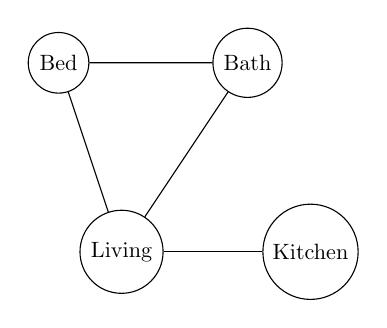
\begin{tikzpicture}[scale=0.8, transform shape]
    \node[shape=circle,draw=black] (1) at (0,3) {Bed};
    \node[shape=circle,draw=black] (2) at (3,3) {Bath};
    \node[shape=circle,draw=black] (3) at (1,0) {Living};
    \node[shape=circle,draw=black] (4) at (4,0) {Kitchen};
    \draw[-] (1) -- (2);
    \draw[-] (1) -- (3);
    \draw[-] (2) -- (3);
    \draw[-] (3) -- (4);
\end{tikzpicture} 
\]
Everytime he enters a room, he chooses one of the doors in that room at random, and moves throuhg it to the next room. The man starts in his bedroom.

\begin{enumerate}
 \item What is the shortest path from the bedroom to the kitchen?
 \item What is the largest path between bed and kitchen (without cycles)?
 \item If the man keeps walking for a very long time, what amount of time he spends in every room?las
 \item What is the expected time that takes the man to visit the kitchen for the first time?
\end{enumerate}

{\bf Solution in discrete time:}

Let $\vec p(t) = (p_1,p_2,p_3,p_3)$ be the vector state defining the probabilities, at time $t$ of finding the drunken man at (bed,bath,living,kitchen), respectively. This can be seen as the following set of stochastic decaying chemical reactions:
\begin{eqnarray*}
 \mbox{Bed}  &\mathrel{\mathop{\rightleftharpoons}\limits^{\delta/2}_{\delta/2}}& \mbox{Bath} \\
  \mbox{Bed}  &\mathrel{\mathop{\rightleftharpoons}\limits^{\delta/2}_{\delta/3}}& \mbox{Living} \\
  \mbox{Bath}  &\mathrel{\mathop{\rightleftharpoons}\limits^{\delta/2}_{\delta/3}}& \mbox{Living} \\
  \mbox{Living}  &\mathrel{\mathop{\rightleftharpoons}\limits^{\delta/3}_{\delta}}& \mbox{Kitchen} 
\end{eqnarray*}


Consider the transition matrix
\[
M = \begin{bmatrix}
1-\delta & \delta/2 & \delta/3 & 0\\
\delta/2 & 1-\delta & \delta/3 & 0\\
\delta/2 & \delta/2 & 1-\delta & \delta\\
0 & 0 & \delta/3 & 1-\delta
\end{bmatrix}\]
such that the evolution in discrete time of the Markov process is given by
\[ \vec p(k+1) = M \cdot \vec p(k) \]
So the full evolution from $t=0$ to $t$ is given by
\[ \vec p (k) = M^k \vec p(0)\]

Matrices as $M$, postive in their values, and such that every column add to 1, are known as stochastic matrices. It can be shown that the largest eigevanlue, in any stochastic matrix, is $\lambda = 1$, and its  eigenvector is a probability vector.

In the current case, it is easy to prove, by substitution, that $\vec p_\infty = (2,2,3,1)/8$ is such eigenvecto. This implies that
\[ \vec p_\infty = M\cdot \vec p_\infty\]
meaning that $\vec p_\infty$ is the stationary solution of the process.

A simple generalization proves that an umbiased random walk on a graph has a steaty state probability that only depends on the degree of each node, and its proportional to it.

{\bf Take home message:} every discrete time homogenous in time Markov process corresponds to a transition (stochastic) matrix, whose $\lambda=1$ eigenvector is the long time limit of the process.

{\bf Continuous time limit:}

We can consider the scaling of this process as we devide the time scale in T units, and send $\delta \to \delta / T$. This process is known as continuous time limit, when $T\to \infty$. In this case
\[  \vec p(k+1) - \vec p(k) = \left( M(\delta/T) - \mathbb{I}\right) \cdot \vec  p(k)\]
resulting in 
\[ \frac {\ud \vec p}{\ud t}  =  \left(M(\delta)-\mathbb I \right) \cdot \vec p\]
Which also shows that the stationary solution is given by 
\[ \frac {\ud \vec p}{\ud t}  = 0 \quad  \Rightarrow   \left(M(\delta)-\mathbb I \right) \cdot \vec p = 0\]
which is the defintion of the eigenvalue $\lambda = 1$ for matrix $M$.

Attention, this eigenvector might not be unique. If it is unique, it is the solution in the long time limit. If it is not unique, then the solution will depend on the initial conditions.


\section{Daniel Bernoulli and smallpox}

Daniel Bernoulli's study of the effect of smallpox in life expentancy and the possibility of innoculation as a vaccination strategy, a debated argument in the Royal Academy of Science in Paris, in the second half of the XVIII century.

Effect of innoculation in Smallpox, 
Royal Academy of Science, Paris, 1760, published in 1766

Scope: calculate the gain in life expectancy at birth if smallpox were to be eliminated as a cause of death. The model assumes a fixed amount of infections every year, so, it is not a model for the infection. Still, it deals with relevant questions in epidemiology.

The model of Bernoulli studied the age dynamics of the entire population in a country, as classified in three groups: susceptibles, immunes and dead\footnote{ As you can see, there is no characterization of those that are currently infected. The reason for this is that the study considered  large time scales, such that the actual infectious period was neglible in that scale, and people were considered to transition immediately between susceptible to immune.}. Susceptible was everyone that had not been in conctact with the disease. Immune was everyone that had passed the disease. Dead were those that died, either from the disease or from other causes. Smallpox could either cause death, or cause life-long immunity. So, it is considered one of the SIR family of models, but rather, in this case, SR model.

 


\[
\begin{tikzpicture}
 \def\dx{0.5}
 \def\oldy{0}
 \def\x{0}
 \foreach \y / \col  [remember=\y as \oldy] in {6/green, 6/red, 6/black}
  {
    \draw[\col,thick] (\x,\oldy+0.1) rectangle (\x+\dx,\y);
    \tikzmath{\he = \y-\oldy-0.1;\points = int( 5*(\y-\oldy)); }
    \foreach \i in {1,...,\points}
    {       \fill[\col] (\x+\dx*random,\oldy+0.1 + \he *random) circle (0.1);
    }
  }
 \def\oldy{0}
 \def\x{1.0}
 \foreach \y / \col  [remember=\y as \oldy] in {4.5/green, 5.3/red, 6/black}
  {
    \draw[\col,thick] (\x,\oldy+0.1) rectangle (\x+\dx,\y);
    \tikzmath{\he = \y-\oldy-0.1;\points = int( 5*(\y-\oldy)); }
    \foreach \i in {1,...,\points}
    {       \fill[\col] (\x+\dx*random,\oldy+0.1 + \he *random) circle (0.1);
    }
  }

   \def\oldy{0}
 \def\x{2.5}
 \foreach \y / \col  [remember=\y as \oldy] in {4/green, 5/red, 6/black}
  {
    \draw[\col,thick] (\x,\oldy+0.1) rectangle (\x+\dx,\y);
    \tikzmath{\he = \y-\oldy-0.1; \points = int( 5*(\y-\oldy)); }
    \foreach \i in {1,...,\points}
    {       \fill[\col] (\x+\dx*random,\oldy+0.1 + \he *random) circle (0.1);
    }
  }
  
 \def\oldy{0}
 \def\x{3.5}
 \foreach \y / \col  [remember=\y as \oldy] in {2.8/green, 4.5/red, 6/black}
  {
    \draw[\col,thick] (\x,\oldy+0.1) rectangle (\x+\dx,\y);
    \tikzmath{\he = \y-\oldy-0.1; \points = int( 5*(\y-\oldy)); }
    \foreach \i in {1,...,\points}
    {       \fill[\col] (\x+\dx*random,\oldy+0.1 + \he *random) circle (0.1);
    }
  }  
  \def\oldy{0}
 \def\x{5}
 \foreach \y / \col  [remember=\y as \oldy] in {2.4/green, 4.2/red, 6/black}
  {
    \draw[\col,thick] (\x,\oldy+0.1) rectangle (\x+\dx,\y);
    \tikzmath{\he = \y-\oldy-0.1;\points = int( 5*(\y-\oldy)); }
    \foreach \i in {1,...,\points}
    {       \fill[\col] (\x+\dx*random,\oldy+0.1 + \he *random) circle (0.1);
    }
  }  
  \def\oldy{0}
 \def\x{6}
 \foreach \y / \col  [remember=\y as \oldy] in {2/green, 4/red, 6/black}
  {
    \draw[\col,thick] (\x,\oldy+0.1) rectangle (\x+\dx,\y);
    \tikzmath{\he = \y-\oldy-0.1;\points = int( 5*(\y-\oldy)); }
    \foreach \i in {1,...,\points}
    {       \fill[\col] (\x+\dx*random,\oldy+0.1 + \he *random) circle (0.1);
    }
  }  
% \def\r{7}
% \def\c{0}
% 
% \draw (\c,\c) circle (\r);
% 
% \foreach \x in {1,2,3,4,5,6}
% {
% \tikzmath{\r=\x/2;\c=\r/sqrt(2);}
% \draw (-\c, \c) circle (\r);
% \draw (\c, -\c) circle (\r); 
% }  
%   
%   \foreach \x / \col in {0/green, 1.2/red, 2.4/black, 3.6/blue, 4.8/orange}
%   {
%     \draw[\col,thick] (\x,0) rectangle (\x+0.8,2);
%     \foreach \i in {1,...,10}
%     {
%       \fill[\col] (\x+0.1*rand,0.1*rand+0.2*\i) circle (0.05);
%     }
%   }
%   \foreach \x in {0,1.2,2.4,3.6,4.8}
%   { 
%     \draw[green,thick] (\x,0) rectangle (\x+0.8,2);
%     \draw[red,thick] (\x,2.2) rectangle (\x+0.8,4.2);
%     \draw[black,thick] (\x,4.4) rectangle (\x+0.8,6.4);
%   }
\end{tikzpicture}
\]



Bernoulli imagined that people born in year $a=0$, could go through the states (un-infected, immune, dead) with certain probabilities \footnote{The transitions between this states were described as a Markov chain, although Markov contribution came centuries later.}
The dynamics relied on the following dynamic parameters:
\begin{itemize}
 \item $\mu(a)$ the rate of death of all causes except smallpox, for an individual of age $a$  
 \item $\beta$ is the {\bf force of infection}: the rate at which susceptible individual get infected
 \item $c = 1-s$ the fraction of individuals infected that dies of smallpox.
\end{itemize}

The Markov chain is described graphically as this:
\[
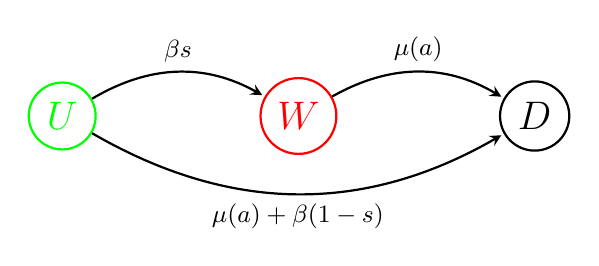
\begin{tikzpicture}[->,>=stealth,shorten >=1pt,auto,node distance=3cm, thick,main node/.style={circle,draw,font=\sffamily\Large\bfseries}]

  \node[main node, green] (U) {$U$};
  \node[main node, red] (W) [right of=U] {$W$};
  \node[main node] (D) [right of=W] {$D$};

  \path[every node/.style={font=\sffamily\small}]
    (U) edge [bend left] node [above] {$\beta s $} (W)
    (U) edge [bend right] node [below] {$\mu(a) + \beta (1-s) $} (D)
    (W) edge [bend left] node [above] {$\mu(a)$} (D);
\end{tikzpicture}
\]

The relevant quantities (dynamic variables) of the model depend on the age of the persons $a$. They are:
\begin{itemize}
 \item $u(a)$ the probability for an individual of being alive and susceptible (uninfected) at age $a$
 \item $w(a)$ the probability for an individual of being alive and immune at age $a$
 \item $d(a)$ is the probability of being dead at age $a$, but since probabilities add up to 1, and there are only three posible states, $d(a) = 1-u(a) -w(a)$.
 \end{itemize}

Considering the rates at which individuals can move from one state to the other, we can compute the contributions of each state in the Master equation. 
The dynamical system derived by Bernoulli is given by:
\begin{eqnarray*}
 \frac{\ud u}{\ud a} &=& -(\beta + \mu(a)) u(a) \\
 \frac{\ud w}{\ud a} &=& \beta (1-c) \mu(a) u(a) -\mu(a) w(a)
\end{eqnarray*}
The interest of Bernoulli was comparing the total amount of persons alive at a given age $u(a)+w(a)$ in the case where $c=0$ (people do not die of smallpox), and $c\neq 0$.

These equations  are recognized as one of the first modern mathematical approaches to mathematical epidemiology. Their solution and Bernoulli conclusions is out of the scope of the present course (if interested see \cite{dietz02}). However, its interpretation and derivation are useful to introduce some probabilistic methods and epidemic concepts. 

The Master Equation provides a powerful framework for analyzing a wide range of phenomena, including chemical reactions, population dynamics, and the behavior of complex systems. By solving the Master Equation, one can obtain the time-dependent probability distribution of the system, which can be used to calculate various statistical quantities of interest, such as the mean and variance of observables. The Master Equation can also be used to study the long-time behavior of the system, such as the emergence of steady-state solutions and the behavior of fluctuations around these solutions.

% Gossiping in science: Bernoulli in letter to Euler, discussing D’Alembert’s critics to his works: 
% \begin{quote}
% (...)je me trouve, trop souvent, injustement traitee dans ses ouvrages, j’ai pris la resolution depuis assez long-temps de ne rien lire qui sorte de sa plume (...) il semble que le succees de cette nouvelle analyse lui fit mal au coeur; il la critique de mille facons, toutes egalement ridicules et aprez l’avoir bien critiquee il se donne pour premier auteur d’une theeorie qu’il n’avoit pas seulement entendu nommer(...) Dolus an virtus quis in hoste requirat.
% \end{quote}
% The latin phrase, from Aeneid, translates to: What matters whether by valour or by stratagem we overcome the enemy?

\section{SIR compartmental models}
The SIR (Susceptible-Infectious-Recovered) model is a widely used mathematical framework for studying the spread of infectious diseases in populations. It  was first introduced by Kermack and McKendrick in a seminal paper published in 1927. They used a system of differential equations to describe the time evolution of the number of individuals in each compartment, and derived an expression for the critical threshold of the disease, above which an epidemic occurs. 
\[
\begin{tikzpicture}[
    declare function={a(\x)=0.75*\x-2;},
    declare function={b(\x)=\x;}
]
  \draw[thick] (0.5,0.4) rectangle (6.35,5.3); % draw the square
\begin{axis}[axis line style={opacity=0},
    domain=0:1,
%     axis lines=middle,
%     axis equal image,
     xtick=\empty, ytick=\empty
%     enlargelimits=true,
%     clip mode=individual, clip=false
]  
\addplot [red, only marks, mark=*, samples=50, mark size=2.5]    {rand};
\addplot [green, only marks, mark=*, samples=100, ma size=2.5]    {rand};
\addplot [black, only marks, mark=*, samples=50, mark size=2.5]    {rand};
%\addplot [thick] {a(x)};
%\addplot [thick] {b(x)};
  % draw labels
  \end{axis}
\end{tikzpicture} \]

A first idealization of what actually happens in an epidemic, is to think of society as a gas of individuals. Each individual can be in one of the following states:
\begin{itemize}
 \item {\bf Susceptible} individuals, who are at risk of becoming infected; 
 \item {\bf Infectious} individuals, who are capable of transmitting the disease to susceptible individuals;
 \item {\bf Recovered} individuals, who have either recovered from the disease and are immune, or have died from the disease, and are removed.
\end{itemize}

Under well mixed assumptions, this individuals-particles move around and interact with each other, occasionally. The process of contagion can be seen as a catalytic chemical reaction, in which the interaction of an Infectious individual with a Susceptible, can induce the latter to turn into infectious with a certain probability:
\begin{eqnarray*}
 S + I &\xrightarrow{\beta}& 2I \\
 I &\xrightarrow{\mu}& R \\
\end{eqnarray*}

Simulation of this process in a computer, relies on Monte Carlo methods, more precisely in action diffusion equations and Gillespie algorithm, that we will study later.
%Their work laid the foundation for the study of infectious disease dynamics, and has since been extended and modified in many ways to incorporate more complex disease transmission mechanisms and population structures.

A mean field probabilistic description can be made, by considering the population to be classified into three different compartments, according to their state:

\[
%     \begin{tikzpicture}
%         % Draw first urn
%         \draw (0,0) rectangle (1.5cm);
%                \foreach \i in {1,...,20}
%             \fill[black] (rand*1.5,rand*1.5) circle (0.1cm);
% 
%          \node at (0,-1.8) {Urn 1};
%         
%         % Draw second urn
%         \draw (5,0) circle (1.5cm);
%         \node at (5,-1.8) {Urn 2};
%         
% %         % Draw third urn
%         \draw (10,0) circle (1.5cm);
%         \node at (10,-1.8) {Urn 3};
   % \end{tikzpicture}
 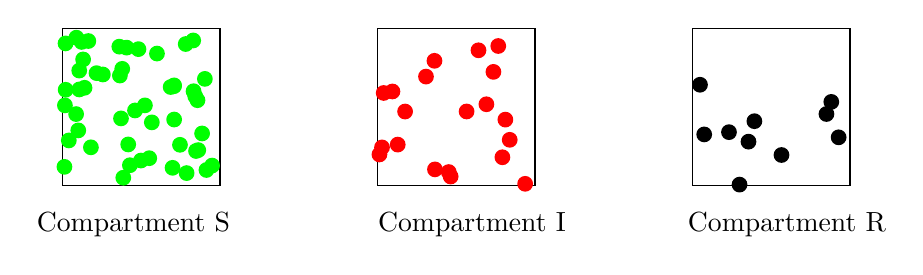
\begin{tikzpicture}
        % Draw first urn
        \draw (0,0) rectangle (2cm,2cm);
        \foreach \i in {1,...,50}
            \fill[green] (random*1.9,random*1.9) circle (0.1cm);
        \node at (0.9,-0.5) {Compartment S};
        
        % Draw second urn
        \draw (4,0) rectangle (6cm,2cm);
        \foreach \i in {1,...,20}
            \fill[red] (4+random*1.9,random*1.9) circle (0.1cm);
        \node at (5.2,-0.5) {Compartment I};
        
        % Draw third urn
        \draw (8,0) rectangle (10cm,2cm);
        \foreach \i in {1,...,10}
            \fill[black] (8+random*1.9,random*1.9) circle (0.1cm);
        \node at (9.2,-0.5) {Compartment R};
    \end{tikzpicture}
    \]
The evolution of the epidemic correspond to the process of changing individuals between compartments, with certain probabilities, as represented in the following diagram:
\[
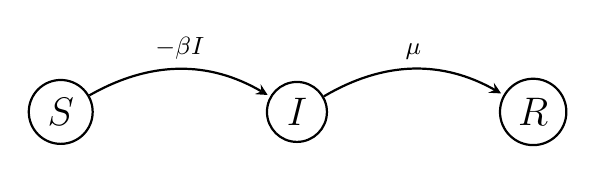
\begin{tikzpicture}[->,>=stealth,shorten >=1pt,auto,node distance=3cm, thick,main node/.style={circle,draw,font=\sffamily\Large\bfseries}]

  \node[main node] (S) {$S$};
  \node[main node] (I) [right of=S] {$I$};
  \node[main node] (R) [right of=I] {$R$};

  \path[every node/.style={font=\sffamily\small}]
    (S) edge [bend left] node [above] {$-\beta I$} (I)
    (I) edge [bend left] node [above] {$\mu$} (R);
\end{tikzpicture}
\]

A key difference with the work of Bernoulli is that the {\it force of infection:} $\beta I(t)$ (the rate at which susceptible individuals contract the disease) is not fixed in time, but proportional to the amount of people infected in the population. This is typical for human-human transmitted diseases in a well mixed population, where the probability of getting infected depends on the chances of meeting an infectious individual. This probability is proportional to the current amount of individuals in that state.

The dynamic variables for this model are:
\begin{itemize}
 \item $S(t)$, the fraction of the population susceptible to contracting the disease
 \item $I(t)$ the fraction that is currently infected and infectious
 \item $R(t) = 1- S(t)  - I(t)$ the fraction that is recovered or deceased.
\end{itemize}

We can write down the master equation of the stochastic process, which defines the evolution in time of $P_{S,I}(t)$, as
\[ \frac{\ud P_{S,I}(t)}{\ud t}  = \beta P_{S+1,I-1}(t) + \mu P_{S,I+1}(t) -\beta P_{S,I}(t) -\mu P_{S,I}(t)\]
By taking the average $S(t)= \frac 1 N \sum_{S,I} S P_{S,I}(t)$ and $I(t)= \frac 1 N \sum_{S,I} I P_{S,I}(t)$, we can obtain the deterministic version of this stochastic process, which characterize the evolution in time of the mean values:
\begin{eqnarray}
\frac{\ud S}{\ud t} &=& -\beta SI  \nonumber \\
\frac{\ud I}{\ud t} &=& \beta SI - \mu I  \label{eq:SIR} \\
\frac{\ud R}{\ud t} &=& \mu I \nonumber
\end{eqnarray}
where, the parameters
\begin{itemize}
 \item $\beta$ is the transmission rate or the rate at which susceptible individuals become infected.
\item $\mu$ is the recovery rate or the rate at which infected individuals recover and become immune.
\end{itemize}

The first equation describes the rate at which susceptible individuals become infected. It assumes that the rate of transmission is proportional to the product of the number of susceptible individuals and the number of infectious individuals, with the proportionality constant $\beta$.

The second equation describes the rate at which infected individuals recover. It assumes that the rate of recovery is proportional to the number of infectious individuals, with the proportionality constant $\mu$. The term $\beta SI$ represents the rate at which susceptible individuals become infected, and the term $\mu I$ represents the rate at which infected individuals recover.

The third equation describes the rate at which individuals recover from the disease and become immune. It assumes that the rate of recovery is proportional to the number of infectious individuals, with the proportionality constant $\mu$.

Sometimes, the equations are written in terms of populations instead of probabilities. You can obtain one from the other by multiplying (dividing) by the population size $N$:
\begin{eqnarray}
\frac{\ud S}{\ud t} &=& -\beta \frac I N S   \nonumber \\
\frac{\ud I}{\ud t} &=& \beta \frac S N I - \mu I  \label{eq:SIR} \\
\frac{\ud R}{\ud t} &=& \mu I \nonumber
\end{eqnarray}
In this case, $\frac  I N$ and $\frac S N$ can be interpreted as the density of infectious/susceptibles individuals, and $\beta$ is still the rate of transmssion contacts per unit time. The {\it force of infection} of a disease is the rate at which susceptible individuals become infected. Said differently, is the probability per unit time of a helathy individual of contracting the disease. In transmissible diseases will be $\beta \frac I N$ and it depends on the size of the infectious population.

These equations are a set of coupled first-order ordinary NON-LINEAR differential equations, which means that the values of $S$, $I$, and $R$ change over time according to the values of $\beta$, $\mu$, and the initial conditions. The nonlinearity, of course, causes some complications.

First epidemics models, however, were linear. For instance, if a model studies a disease that apperas in the population at a fixed rate, lets say, skin cancer (non transmissible), then a deterministic model looks like:
\begin{eqnarray}
 \frac{\ud S}{\ud t} &=& b S -\beta S -d S  \nonumber \\
\frac{\ud I}{\ud t} &=& \beta S - \mu I  -d_I I\label{eq:SIRlinear} \\
\frac{\ud R}{\ud t} &=& \mu I - d_R R \nonumber
\end{eqnarray}
Notice that this equations are linear, therefore an scaling by $N$ or any other factors is irrelevant.



\subsection{Deterministic epidemics from master equation}

Previous deterministic equations are similar in spirit to the master equation, but actually simpler and quite different in nature. While the stochasti process needs a full description of the probabilities of every possible state of the system, the SIR equations describe determinisic mean values of this process. Intuitively, following the law of large numbers, one expect that such large epidemics will be better described by the deterministic case.

Let us show how deterministic equations are obtained by averaging the master equation. Consider the SIR epidemic process. The full space of the stochastic process is given by the dots in the figure, laying in the area $S+I\leq N$.
\[
\begin{tikzpicture}[scale=0.5]
  \draw[->] (-1,0) -- (21,0) node[right] {$S$};
  \draw[->] (0,-1) -- (0,21) node[above] {$I$};
  \foreach \x in {0,2,...,20}
    {\tikzmath{\maxy = 20-\x;}
    \foreach \y in {0,2,...,\maxy}
      \filldraw[black] (\x,\y) circle (2pt);}
  \draw[->, ultra thick, red] (10,4) -- (8,6);
  \draw[->, ultra thick, green] (10,4) -- (10,2);
  \draw[->, thick,dashed, red] (12,2) -- (10.5,3.5);
  \draw[->, thick,dashed, green] (10,6) -- (10,4.5);
  \draw[dashed] (0,20) -- (20,0);
\end{tikzpicture} \]
The red arrow exemplifies the contagion process, and the green arrow the recovery process. So, from any given state $(S,I)$ there are two possible transitions
\begin{eqnarray*}
 (S , I) &\xrightarrow{W_{I}}& (S-1,I+1) \qquad (S,I) \xrightarrow{W_R} (S,I-1)  \\
\end{eqnarray*}
with transition rates given by
\[W_{I} = \beta \frac I N S  \qquad W_{R} = \mu I\]
The master equations reads
\[ \frac{\ud P_t(S,I)}{\ud t} = \beta  \frac {I-1} N (S+1) P_t(S+1,I-1) +  \mu (I+1) P_t(S,I+1) - \beta  \frac {I} N {S} P_t(S,I) -  \mu (I+1) P_t(S,I)\]
Multiplying by $S$ and tracing over $S$ and  $I$
\begin{eqnarray*}
 \frac{\ud \langle S \rangle}{\ud t} &=& \beta  \sum_{S,I} \frac {I-1} N S (S+1) P_t(S+1,I-1) +  \mu \sum_{S,I}  S (I+1) P_t(S,I+1) - \\
 && - \beta  \sum_{S,I} \frac {I} N {S^2} P_t(S,I) -  \mu\sum_{S,I}  S I P_t(S,I)
\end{eqnarray*}
It suffices to assume that $P(S,I)\equiv 0$ whenever either of the arguments is negative or $S+I>N$, to change variables and obtain:
\begin{eqnarray*}
 \frac{\ud \langle S \rangle}{\ud t} &=& \beta  \sum_{\tilde S,\tilde I} \frac {I} N (S-1) S P_t(S,I) +  \mu \sum_{S,\tilde I}  S I P_t(S,I) - \\
 && - \beta  \sum_{S,I} \frac {I} N {S^2} P_t(S,I) -  \mu\sum_{S,I}  S I P_t(S,I) \\
 &=& - \beta \frac 1 N \langle S I \rangle
\end{eqnarray*}

Repeating for the average of $I$, we get the equations
\begin{eqnarray*}
 \frac{\ud \langle S \rangle}{\ud t}  &=& - \beta \frac 1 N \langle S I \rangle \\
  \frac{\ud \langle I \rangle}{\ud t}  &=& + \beta \frac 1 N \langle S I \rangle - \mu \langle I\rangle
\end{eqnarray*}
which are similar but yet not the same as the SIR model equations. A further assumption $\langle S I \rangle \simeq \langle S \rangle  \langle I \rangle $ is required to reproduce SIR model. This assumption shall be good if the variables S and I are actually independent, which is not mathematically the case. But it shall be a good approximation is the distribution $P_t(S,I)$ is sharply picked arround its mean values. This is the case for large systems, where we expect a sort of law of large numbers to concentrate the stochastic process on its typical values.


\subsection{Short time limit}

In the early stages of an epidemic, when the number of infected individuals is small compared to the total population size, the SIR model can be approximated by a linear differential equation. %This linearized SIR model predicts that the number of infected individuals grows exponentially at a rate proportional to the number of susceptible individuals, until a significant proportion of the population becomes infected and the epidemic enters a saturation phase.
Suppose that the initial number of infected individuals is small compared to the total population size, i.e., $I(0) \sim 1/N$, where $N$ is the total population size. Then, the number of susceptible individuals can be approximated as $S(t) \simeq 1$, and the number of recovered individuals can be approximated as $R(t) \sim 1/N$.

Under these assumptions, the dynamics of the infected compartment can be approximated by the following linear differential equation:
\begin{equation}
    \frac{dI}{dt} = \beta S(t) I(t) - \mu I(t),
\end{equation}
where $\beta$ is the transmission rate, $\mu$ is the recovery rate, and $I(t)$ is the fraction of infected individuals at time $t$. During the initial epidemic phase, when few cases still exists compared to the population size, we can approximate $S(t) = S(0) = 1$, and write the linear equation:
\begin{equation}
    \frac{dI}{dt} = \lambda I(t), \qquad \mbox{where }   \lambda = \beta - \mu.
\end{equation}
The solution to this linear differential equation is an exponential function of the form:
\begin{equation}
    I(t) = I(0) \exp(\lambda t).
\end{equation}
The exponential solution of the SIR model in the low prevalence linear phase shows that the number of infected individuals changes exponentially, growing when $\beta>\mu$, and decreasing when $\beta<\mu$.  This exponential growth phase is characteristic of the beginning of an epidemic, when the number of infected individuals is small compared to the total population size and the epidemic has not yet reached a significant proportion of the population. 

The basic reproduction number $R_0$, is the expected number of new infections created by every single infected individual, in the early exponential phase of an epidemic. Since $\mu$ is the recovery rate, $\tau = 1/\mu$ is the expected duration of the infection on an individual. Since $\beta$ is the rate of new cases, $R_0 = \beta \tau = \beta/\mu$ is the average number of new cases created by an infected individual during the period in which it is actively infectious. Notice that the criteria $\lambda \lessgtr 0$ is equivalent to $R_0 \lessgtr 1$.

%The duration and magnitude of the exponential growth phase depend on the initial conditions and the parameters of the model, such as the transmission rate and recovery rate.

\subsection{Infinite time limit}

Properties of SIR equations. Since the total amount of studied subjects remain invariant, only their categories changes, $S(t)+I(t)+R(t) =1$. This can also be proven by adding (\ref{eq:SIR}). Furthermore, since \[ S'(t)+I'(t) = -\mu I(t)\] is a decreasing non negative function, it converges to a limit $S_\infty + I_\infty$ in $t\to\infty$. Moreover, it is easy to see that $I_\infty$ can only be zero, so $S+I \to S_\infty$.

Integration of the previous equation results in
\[ 1 - S_\infty  = \mu \int_0^\infty I(t)\ud t
\]
The first number $S_0+I_0 = 1$ comes from assuming that all the population is originally in the states S or I.

Dividing the equation for $S'(t)$ by $S(t)$, we get
\[ \frac{ \ud \log S(t)}{\ud t}  =  -\beta I(t) \quad \mbox{that integrating }\quad  \log(S_\infty / S_0) = -\beta \int_0^\infty I(t)\ud t\] This results in a relation for the final amount of susceptible individuals
\[\log(S_0 / S_\infty)  = \frac \beta \mu (1-S_\infty) = R_0 (1-S_\infty) \]
that is called the {\it final size relation} for the epidemic. If the variables are kept extensive $\tilde S(t) = N S(t), \tilde I(t) \ldots $, the final relation reads
\begin{equation}
 \log(\tilde S_0 / \tilde S_\infty)  =  R_0 (1-\frac {\tilde S_\infty} N) \label{eq:Sinf} 
\end{equation}
which is a useful relation between the basic reproduction number and the final size of the epidemic. 

The total number of infected people in the population is given by $N-\tilde S_\infty$, and the fraction $1-S_\infty$ or $1-\frac {\tilde S_\infty }N$ is called the {\it attack rate}, although it is not a rate, but a fraction.

Another conclusion from (\ref{eq:Sinf}) is that $S_\infty>0$, and so, in every epidemic there is always a fraction of the population that will not be infected.

While the recovery rate $\mu$ is generally simple to estimate from studies on infected individuals. However the contact rate $\tilde \beta = \beta/N$ is much harder. Direct calculation of $\beta$, or of $R_0 =\beta/\mu$ can be difficult, while a post facto analysis of the epidemic through serological studies, can provide estimation for $S_\infty$, and through (\ref{eq:Sinf}), to $R_0$ and $\beta$.

\[
   \begin{tikzpicture}[
    scale=4,
    axis/.style={very thick, ->},
    important line/.style={thick},
    dashed line/.style={dashed, thin},
    pile/.style={thick, ->, shorten <=2pt, shorten
    >=2pt},
    every node/.style={color=black}
    ]
        % Draw grid
%        \draw[step=0.2,gray,thin] (0,0) rectangle (1,1);
%        \draw[thick,->] (0,0) -- (3.1,0) node[anchor=north west] {X};
%        \draw[thick,->] (0,0) -- (0,3.1) node[anchor=south east] {Y};
          \draw[axis] (-0.1,0)  -- (1.0,0) node(xline)[right] {$S$};
        \draw[axis] (0,-0.1) -- (0,1.0) node(yline)[above] {$I$};
        %\draw[thick] (0,0) rectangle (1,1);        % Draw vectors
        \foreach \x in {0.05,0.1,...,0.95}
            {\tikzmath{\e = 1.0-\x;}
            \foreach \y in {0.05,0.1,...,\e}
            {
                  \tikzmath{\dx = -0.5* \x * \y;
                            \dy =  -1* \dx -0.6* \y;
                             \norm = {sqrt(100*\dx*\dx + 100*\dy*\dy)};
                             \dxn = 10*0.05*\dx/(0.01+\norm);
                             \dyn = 10*0.05*\dy/(0.01+\norm);
                            }
                  \draw[->,thick] (\x,\y) -- ( \x+\dxn, \y+\dyn );}}
          \draw[axis] (1.9,0)  -- (3.0,0) node(xline)[right] {$S$};
        \draw[axis] (2.0,-0.1) -- (2.0,1.0) node(yline)[above] {$I$};
        %\draw[thick] (0,0) rectangle (1,1);        % Draw vectors
        \foreach \x in {0.05,0.1,...,0.95}
            {\tikzmath{\e = 1.0-\x;}
            \foreach \y in {0.05,0.1,...,\e}
            {
                  \tikzmath{\dx = -0.5* \x * \y;
                            \dy =  -1* \dx -0.2* \y;
                             \norm = {sqrt(100*\dx*\dx + 100*\dy*\dy)};
                             \dxn = 10*0.05*\dx/(0.01+\norm);
                             \dyn = 10*0.05*\dy/(0.01+\norm);
                            }
                  \draw[->,thick] (2+\x,\y) -- ( 2+\x+\dxn, \y+\dyn );}}
                  
\end{tikzpicture}
\]

A similar procedure as the one we carried, but taken up to time $t$ instead of $\infty$, results in a parametric relation between $S(t)$ and $I(t)$:
\begin{equation} 
I(t) +S(t) - \frac \mu\beta \log S(t) = 1- \frac \mu\beta \log S_0 \label{eq:SIintime}
\end{equation}

This trajectories correspond to the flux lines in the diagram of $I$ vs $S$, using the vector defined by the right hand side of (\ref{eq:SIR}), normalized.

The maximum number of infectives at any time is the number of infectives when the derivative of $I$ is zero, that is, when $S = \mu /\beta$ . This maximum is obtained by replacing this value into (\ref{eq:SIintime}) as
\[ I_{max} =  I_0 +S_0 - \frac \mu\beta \log S_0  - \frac \mu\beta +\frac \mu\beta \log \frac{\mu}{\beta} 
\]

\subsection{Epidemics terminology}

A clear definition of terms is essential for the correct handling of epidemics. At the onset of any epidemic and in particular for emerging diseases, a clear statement of what is going to be consider a ``case'', a ``death caused by the disease'', a primary or secondary case, among others, is essential for a meaningful collection of statistical data, which is a key aspect of epidemiology.

Following WHO summary of terms for COVID (COVID-19, GLOSSARY: OUTBREAKS AND EPIDEMICS, A resource for journalists and communicators), here comes a selected list of useful terms related to epidemics:
\begin{itemize}
\item Emerging disease: An unknown or newly appeared disease, usually of the infectious or communicable type.
\item Reemerging disease: Resurgence or increase in the incidence of infectious or
communicable diseases that were considered to be already under control.
\item Seasonality of disease: Regular pattern of variation in the occurrence of some diseases
(for example, the flu) during different seasons of the year.
\item Incidence: The number of new cases of a disease in a population in a given period.
Incidence measures the speed at which new cases occur during a given period in a specific
population—for example, the number of new cases of HIV infection in gay men in a country in 2019.
 \item Prevalence: The total number of people who have a disease (new and existing cases)
in a population or in a given place at a given time. Prevalence is an indicator of the
magnitude of a disease—for example, the total number of people with tuberculosis in
a country in 2019. Incidence and prevalence are essentially different ways of measuring
the frequency of disease. The relationship between them varies from disease to disease.
\item Attack rate: Number of people who contract a disease out of the entire group of people exposed to the disease. Expressed as a percentage.
\item Agent: A microorganism, chemical substance, or form of radiation whose
presence, excessive presence, or relative absence is essential for the occurrence of
a disease Agents may be biological (living organisms, such as viruses and bacteria) and
non-biological (chemicals, such as pesticides, and physical phenomena, such as radiation).
\item Case-fatality rate: The percentage of people affected by a disease or a particular event who die in a given period. Frequently used to describe the severity of an epidemic.
\item Contact: A person who has been in contact with an infected person (case) such that he/she is considered to have had significant exposure and is therefore at risk of infection.
\item Contagious or infectious: Terms that are often used interchangeably but that have subtle differences in meaning. “Contagious” is related to direct or indirect spread from person to person. The flu, for example, is very contagious, but Ebola is not. “Infectious” means that contact with a small amount of virus can cause disease. Ebola, for example, is very infectious.
\item Host: A person or other living animal, including birds and arthropods, that affords
subsistence or lodgment to an infectious agent under natural conditions.
\item Exposure: Contact with an infectious agent or a risk factor that can cause a disease.
Exposure has two dimensions: degree or level, and duration.
\item Incidence rate: Rate of new cases in a population. The numerator is the number of
new events that they occur in a given period. The denominator is the population at risk of
experiencing the event of interest during this period.
\item Infectious period: Period of time during which a person can transmit a disease. This period may precede the onset of symptoms and may last longer than the symptoms.
\item Latent period: Time that elapses from exposure to an agent until the date that
a person can transmit a disease (this is the period that immediately precedes the
infectious period).
\item Mortality rate: Percentage of people in a population who die out of the total
population. May be expressed per 100, 1,000, or another number.
\item Virulence: The ability of an infectious agent to produce severe and fatal cases. The measure of virulence is the ratio of the number of severe and fatal cases to total overt cases.
\item Basic reproduction number (R0): The spread of a disease in a population (especially in epidemics) depends on the basic reproduction number (or R0) and the generation time (usually established on the basis of the serial interval). The R0 is the number of people to whom an
infected person can transmit the disease or the number of secondary cases that each
primary case generates on average (during the contagious period).
\item Generation time: the time between the  onset of infection in the primary case and the
onset of infection in a secondary case (i.e., a case infected by the primary case)
\item Serial interval: In practical terms, this is the time between the onset of the disease
in the primary case and the onset of the disease in the secondary case: the longer the serial interval, the more time there is to act on the problem, implement prevention and control measures, and, therefore, the better the chances of containing the epidemic.
The shorter the generation time, the more difficult it is to control the outbreak.
\item Isolation means separating sick or infected people from others to prevent infection from
spreading.
\item Quarantine means restricting the movement of healthy people who may have
been exposed to a virus but are not sick.
\item Herd immunity: Indirect protection against disease that results from a sufficient number
of individuals in a community having immunity to that disease. With enough immune individuals, the transmission of a disease can be reduced, thus limiting the potential for any one individual to be exposed to it. Generally, PAHO recommends vaccination coverage of $95\%$ or more to ensure herd immunity. Herd immunity does not apply to diseases such as tetanus that are
not spread via person-to-person contact.
\end{itemize}

\section{SIS model and epidemic thresholds}

SIR epidemics mimic diseases that generate immunity, that is, that you can not take twice. This is the case of many (most) diseases, but it is not the case of many others, as, typically, sexually transmitted diseases, as clamydia and gonorrhea. This diseases are actually best represented by SIS types of models. These are characterized by the transitions
\begin{eqnarray*}
 S + I &\xrightarrow{\beta}& 2I \\
 I &\xrightarrow{\mu}& S \\
\end{eqnarray*}
and the corresponding determinisic equations
\begin{eqnarray}
\frac{\ud S}{\ud t} &=& -\beta SI   + \mu I\nonumber \\
\frac{\ud I}{\ud t} &=& \beta SI - \mu I  \label{eq:SIS}
\end{eqnarray}
While the epidemic phase $I > 0$ in an SIR model last a finite period of time, recurrent diseases can sustain epidemics for infinite time, normally referred as endemic phase. While SIS model is also non linear, the steady state can be easily deduced by setting to zero the time derivatives:
\begin{eqnarray}
\frac{\ud S}{\ud t}\equiv 0 &=& -\beta SI   + \mu I\nonumber \\
\frac{\ud I}{\ud t}\equiv  0  &=& \beta SI - \mu I  \label{eq:SIS}
\end{eqnarray}
resulting in the equilibrium solution
\[ S_{eq} = \frac \mu  \beta \qquad  I_{eq} = 1-S_{eq} = \frac{\beta - \mu } \beta\]
Of course this values will be meaningful if they are in the $[0,1]$ range, meaning that only the case $\beta > \mu$ will generate an endemic phase.
The value $\beta / \mu = 1$, corresponding also with $R_0=1$, defines the threshold above/below which endemic states do/do not exist.

Sometimes, SIS is a too simplistic approach, since almost every disease generates some level of immunity, although it can be lost in time.

\section{And beyond}

Reasons why deterministic description of epidemics is a very narrow approach:
\begin{itemize}
 \item Well mixed systems are non realistic. Human behavior is a mixture of repetitive patterns (go to school, visit your parents, etc) and random interactions (in the public transport system), also influenced by distance constraints. The network of human contacts is best modelled by a dynamic network with rather stable clusterized subnetworks and random links whose probability decays with distance.
 \item Fluctuations: as the whole approach relies implicitly in the law of large numbers, fluctuations are completely ignored. Epidemic processes like SIS  have an absorbing state, i.e. $I=0$. Even epidemics above the epidemic threshold can be suppressed by fluctuations.
 \item Implies memorlyless processes. The assumption that recovery times follow an exponential distribution is motivated by its mathematical convenience rather than its epidemiological plausibility.
\end{itemize}



\section{Homework}

\begin{enumerate}

 \item  Find out the incidence in a year and the prevalence of HIV in Cuba, China, India, USA, Haiti, Nigeria, Spain.

\item Consider the linear model in (\ref{eq:SIRlinear}) as a model for skin cancer.
\begin{enumerate}
 \item What are reasonable values for the constants $b$ and $d$?
 \item Assume that half of people with skin cancer get cure, and half die of this condition. What can we say about $\mu$ and $d_I$?
 \item Force of infection (not actually infection, but developing the disease), lets say is $\beta = 10^{-4}$. And for those who die of this disease, the average time from contraction to death is 1 year. Compute how many individuals are currently living with skin cancer.
 \end{enumerate}

 \item Show that the number of infectious individuals always go to zero in the long time limit of the SIR model.

 \item Consider $\theta  = \beta / \mu$ and using
 \[ I = N -R-S_0 e^{-\theta R(t)}\]
 show that the maximum number of infectious people occurs exactly at $S(t)= 1/\theta$. Show also that in the long time limit not everybody was infected. {\bf Comment:} The first result can be derived in many different ways, some easier than the one proposed.

 \end{enumerate}
